\documentclass[12pt,a4paper,UTF8]{article}
\usepackage{ctex}
\usepackage{amsmath,amscd,amsbsy,amssymb,latexsym,url,bm,amsthm}
\usepackage{epsfig,graphicx,subfigure}
\usepackage{enumitem,balance}
\usepackage{wrapfig}
\usepackage{mathrsfs,euscript}
\usepackage[usenames]{xcolor}
\usepackage{hyperref}
\usepackage[vlined,ruled,linesnumbered]{algorithm2e}
\usepackage{caption}
\hypersetup{colorlinks=true,linkcolor=black}

\newtheorem{theorem}{Theorem}
\newtheorem{lemma}[theorem]{Lemma}
\newtheorem{proposition}[theorem]{Proposition}
\newtheorem{corollary}[theorem]{Corollary}
\newtheorem{exercise}{Exercise}
\newtheorem*{solution}{Solution}
\newtheorem{definition}{Definition}
\theoremstyle{definition}

\renewcommand{\thefootnote}{\fnsymbol{footnote}}

\newcommand{\postscript}[2]
 {\setlength{\epsfxsize}{#2\hsize}
  \centerline{\epsfbox{#1}}}

\renewcommand{\baselinestretch}{1.0}

\setlength{\oddsidemargin}{-0.365in}
\setlength{\evensidemargin}{-0.365in}
\setlength{\topmargin}{-0.3in}
\setlength{\headheight}{0in}
\setlength{\headsep}{0in}
\setlength{\textheight}{10.1in}
\setlength{\textwidth}{7in}
\makeatletter \renewenvironment{proof}[1][Proof] {\par\pushQED{\qed}\normalfont\topsep6\p@\@plus6\p@\relax\trivlist\item[\hskip\labelsep\bfseries#1\@addpunct{.}]\ignorespaces}{\popQED\endtrivlist\@endpefalse} \makeatother
\makeatletter
\renewenvironment{solution}[1][Solution] {\par\pushQED{\qed}\normalfont\topsep6\p@\@plus6\p@\relax\trivlist\item[\hskip\labelsep\bfseries#1\@addpunct{.}]\ignorespaces}{\popQED\endtrivlist\@endpefalse} \makeatother

\begin{document}
\noindent

%========================================================================
\noindent\framebox[\linewidth]{\shortstack[c]{
\Large{\textbf{Lab02-Divide and Conquer}}\vspace{1mm}\\
CS214-Algorithm and Complexity, Xiaofeng Gao, Spring 2020.}}
\begin{center}
\footnotesize{\color{red}$*$ If there is any problem, please contact TA Yiming Liu.}

% Please write down your name, student id and email.
\footnotesize{\color{blue}$*$ Name:Yijia Diao(刁义嘉)  \quad Student ID:518030910146 \quad Email: diao\_yijia@sjtu.edu.cn}
\end{center}

\begin{enumerate}
    \item
    \textbf{Quicksort} is based on the Divide-and-Conquer method. Here is the two-step divide-and-conquer process for sorting a typical subarray $A[p \ldots r]$:
    \begin{enumerate}

    	\item
    	\textbf{Divide:} Partition the array $A[p \ldots r]$ into two subarrays $A[p \ldots q-1]$ and $A[q+1 \ldots r]$ such that each element of $A[p \ldots q-1]$ is less than or equal to $A[q],$ which is, in turn, less than or equal to each element of $A[q+1 \ldots r].$ Compute the index $q$ as part of this partitioning procedure.
    	
    	\item
    	\textbf{Conquer:} Sort $A[p \ldots q-1]$ and $A[q+1 \ldots r]$ respectively by recursive calls to Quicksort.
    	
    \end{enumerate}
    Write down the recurrence function $T(n)$ of QuickSort and compute its time complexity.

    {\color{purple}Hint: At this time $T(n)$ is split into two subarrays with different sizes (usually), and you need to describe its recurrence relation by the sum of two subfunctions plus additional operations.}
    \begin{solution}
    	When $ q = k , 1\leq k \leq n$, and since the time complexity of divide is $ O(n) $(proofed in Lab01), the recurrence function of QuickSort is
    	$$ T(n) = T(k-1) + T(n-k) + O(n) $$
    	Now compute its time complexity by cases:
    	\begin{enumerate}
    		\item[(1)] \textbf{Best case}: the recurrence function is:
    		$$ T(n) = 2T(\lceil n/2\rceil) + O(n) $$
    		According to Master Theorem, since $ d=1 = \log_2 2 = \log_b a$, $ T(n) = O(n\log n) $.
    		\item[(2)] \textbf{Worst case}: the recurrence function is:
    		$$ T(n) = T(0) + T(n-1) + O(n) $$
    		After accumulation, $ T(n) = O(\frac{(n + 2)(n-1)}{2}) = O(n^2) $
    		\item[(3)] \textbf{Average case}: according to the definition of average time complexity, the recurrence function is:
    		\begin{align*}
    		T(n) = \sum_{k = 1}^{n} \Pr(i=k)(O(n)+T(i-1)+T(n - i))
    		\end{align*}
    		The Master Theorem does not apply to this case. According to Lab01 Problem1, $ T(n) = O(n\log n) $.
    	\end{enumerate} 
    \end{solution}

    \item
    \textbf{MergeCount}. Given an integer array $A[1 \ldots n]$ and two integer thresholds $t_l \le t_u$, Lucien designed an algorithm using divide-and-conquer method (As shown in Alg.~\ref{Alg-MergeCount}) to count the number of ranges $(i,j)$ ($1 \leq i \leq j \leq n$) satisfying
    \begin{equation}\label{Eqn-MergeCount}
    t_l \leq \sum_{k=i}^{j}{A[k]} \leq t_u.
    \end{equation}

    Before computation, he firstly constructed $S[0 \ldots n+1]$, where $S[i]$ denotes the sum of the first $i$ elements of $A[1 \ldots n]$. Initially, set $S[0]=S[n+1]=0$, $low=0$, $high=n+1$.

\begin{minipage}[t]{0.90\textwidth}
	\begin{algorithm}[H]
		%\algsetup{footnotesize}
		%\scriptsize
		\KwIn{$S[0,\cdots,n+1]$, $t_l$, $t_u$, $low$, $high$.}
		\KwOut{$count$ = number of ranges satisfying Eqn.~\eqref{Eqn-MergeCount}.}
		\BlankLine
		\caption{MergeCount($S$, $t_l$, $t_u$, $low$, $high$)}
		\label{Alg-MergeCount}
		
		$count \leftarrow 0$; $mid\leftarrow \lfloor \frac{low+high}{2} \rfloor$\;
		
		\lIf{$mid=low$}{
			\Return{$0$}
		}
		
		$count\leftarrow MergeCount(S, t_l, t_u, low, mid)+ MergeCount(S, t_l, t_u, mid, high)$\;
		
		\For{$i = low$ \textbf{to} $mid-1$}{
			$m \leftarrow \left \{ \begin{array}{ll}
            \min\{m \mid S[m]-S[i] \ge t_l, m \in [mid, high-1]\}, & \text{if exists}\\
            high, & \text{if not exist}
            \end{array}\right.$\;
			
			$n \leftarrow \left \{ \begin{array}{ll}
            \min\{n \mid S[n]-S[i] > t_u, n \in [mid, high-1]\}, & \text{if exists}\\
            high, & \text{if not exist}
            \end{array}\right.$
			\tcp*[r]{\color{blue}BinarySearch is used to find $m$, $n$}
			$count \leftarrow count+n-m$\;
		}
		$Merge(S,low,mid-1,high-1)$  \tcp*[r]{\color{blue}Merge is used for two sorted arrays}
		
		\Return{$count$}\;
		
	\end{algorithm}
\end{minipage}

    {\color{purple}\textbf{Example:} Given $A = [1,-1,2]$, $lower = 1$, $upper = 2$, return 4. The resulting four ranges should be $(1,1)$, $(1,3)$, $(2,3)$, and $(3,3)$.}

    Is Lucien's algorithm correct? Explain his idea and make correction if needed. Besides, compute the running time of Alg.~\ref{Alg-MergeCount} (or the corrected version) by recurrence relation. {\color{blue}(Note: we can't implement Master's Theorem in this case. Refer Reference06 for more details.)}
    \begin{solution}
    	Lucien's algorithm is \textbf{not correct}. The error is in Line \textbf{2}; the correction should be:\\
    	\lIf{$mid=high$}{
    		\Return{$0$}
    	}
    	\textbf{Idea}: Alg.~\ref{Alg-MergeCount} uses top-down Divide-and-Conquer in general.\\ It divides input array in half, and do counting and merging in both sub-arrays; the merge operation is equivalent to Mergesort in sub-arrays.\\ After returning to the recursive call function, it make use of the ordered state of the latter sub-array, to count between the former and latter sub-array; add this result and sub-arrays' counting number, then get the counting number of input array. Before returning, finish the merge step so that input array would be sorted. 
    	
    	Suppose the time complexity of corrected Alg.~\ref{Alg-MergeCount} is $ T(n) $.\\
    	Between line \textbf{4} and line \textbf{7}, the time complexity of the \textbf{best case} is $ \frac{n}{2}\cdot2\cdot1 = O(n)$, the \textbf{worst and average case} is $ \frac{n}{2}\cdot2\log\frac{n}{2} = O(n\log n) $; the time complexity of Merge is O(n). Therefore, we compute $ T(n) $ by case:
    	\begin{enumerate}
    		\item[(1)] \textbf{Best case}: the recurrence function is:
    		$$T(n) = 2T(\lceil \frac{n}{2} \rceil) + O(n)$$
    		According to Master Theorem, since $ 1 = \log_2 2 $, $ T(n) = O(n\log n) $.
    		\item[(2)] \textbf{Worst and Average case}: the recurrence function is:
    		$$T(n) = 2T(\lceil \frac{n}{2} \rceil) + O(n\log n)$$
    		Then we do iteration:
    		\begin{align*}
    		T(n) &= 2(2T(\lceil \frac{n}{4} \rceil) + O(\frac{n}{2}\log \frac{n}{2})) + O(n\log n) = 2^2T(\lceil \frac{n}{4} \rceil) + 2^1O(\frac{n}{2}\log \frac{n}{2}) + 2^0O(n\log n)\\
    		&= \cdots\\
    		&= \sum_{i = 0}^{k} 2^{k-i}\cdot O(2^i\cdot i), k = \log n
    		\end{align*}
    		So we have$ T(n) = O(2^k\cdot k^2) = O(n\log^2 n) $.
    	\end{enumerate}
    	We can conclude that the time complexity of Alg.~\ref{Alg-MergeCount} is $ O(n\log^2 n) $.
    \end{solution}

    \item
    \textbf{Batcher's odd-even merging network.} In this problem, we shall construct an \textbf{\textit{odd-even merging network}}. We assume that $n$ is an exact power of $2$, and we wish to merge the sorted sequence of elements on lines $\left\langle a_{1}, a_{2}, \ldots, a_{n}\right\rangle$ with those on lines $\left\langle a_{n+1}, a_{n+2}, \ldots, a_{2n}\right\rangle .$ If $n=1$, we put a comparator between lines $a_{1}$ and $a_{2}$. Otherwise, we recursively construct two odd-even merging networks that operate in parallel. The first merges the sequence on lines $\left\langle a_{1}, a_{3}, \ldots, a_{n-1}\right\rangle$ with the sequence on lines $\left\langle a_{n+1}, a_{n+3}, \ldots, a_{2n-1}\right\rangle$ (the
    odd elements). The second merges $\left\langle a_{2}, a_{4}, \ldots, a_{n}\right\rangle$ with $\left\langle a_{n+2}, a_{n+4}, \ldots\right.$
    $\left.a_{2n}\right\rangle$ (the even elements). To combine the two sorted subsequences, we put a comparator between $a_{2i}$ and $a_{2i+1}$ for $i=1,2, \ldots, n-1$.
    \begin{enumerate}
    	\item Replace the original Merger (taught in class) with Batcher's new Merger, and draw $2n$-input sorting networks for $n=8, 16, 32, 64$. {\color{blue}(Note: you are not forced to use Python Tkinter. Any visualization tool is welcome for this question.)}
    	
    	\begin{figure}[htbp]
    		\begin{minipage}[h]{0.48\textwidth}
    			\centering
    			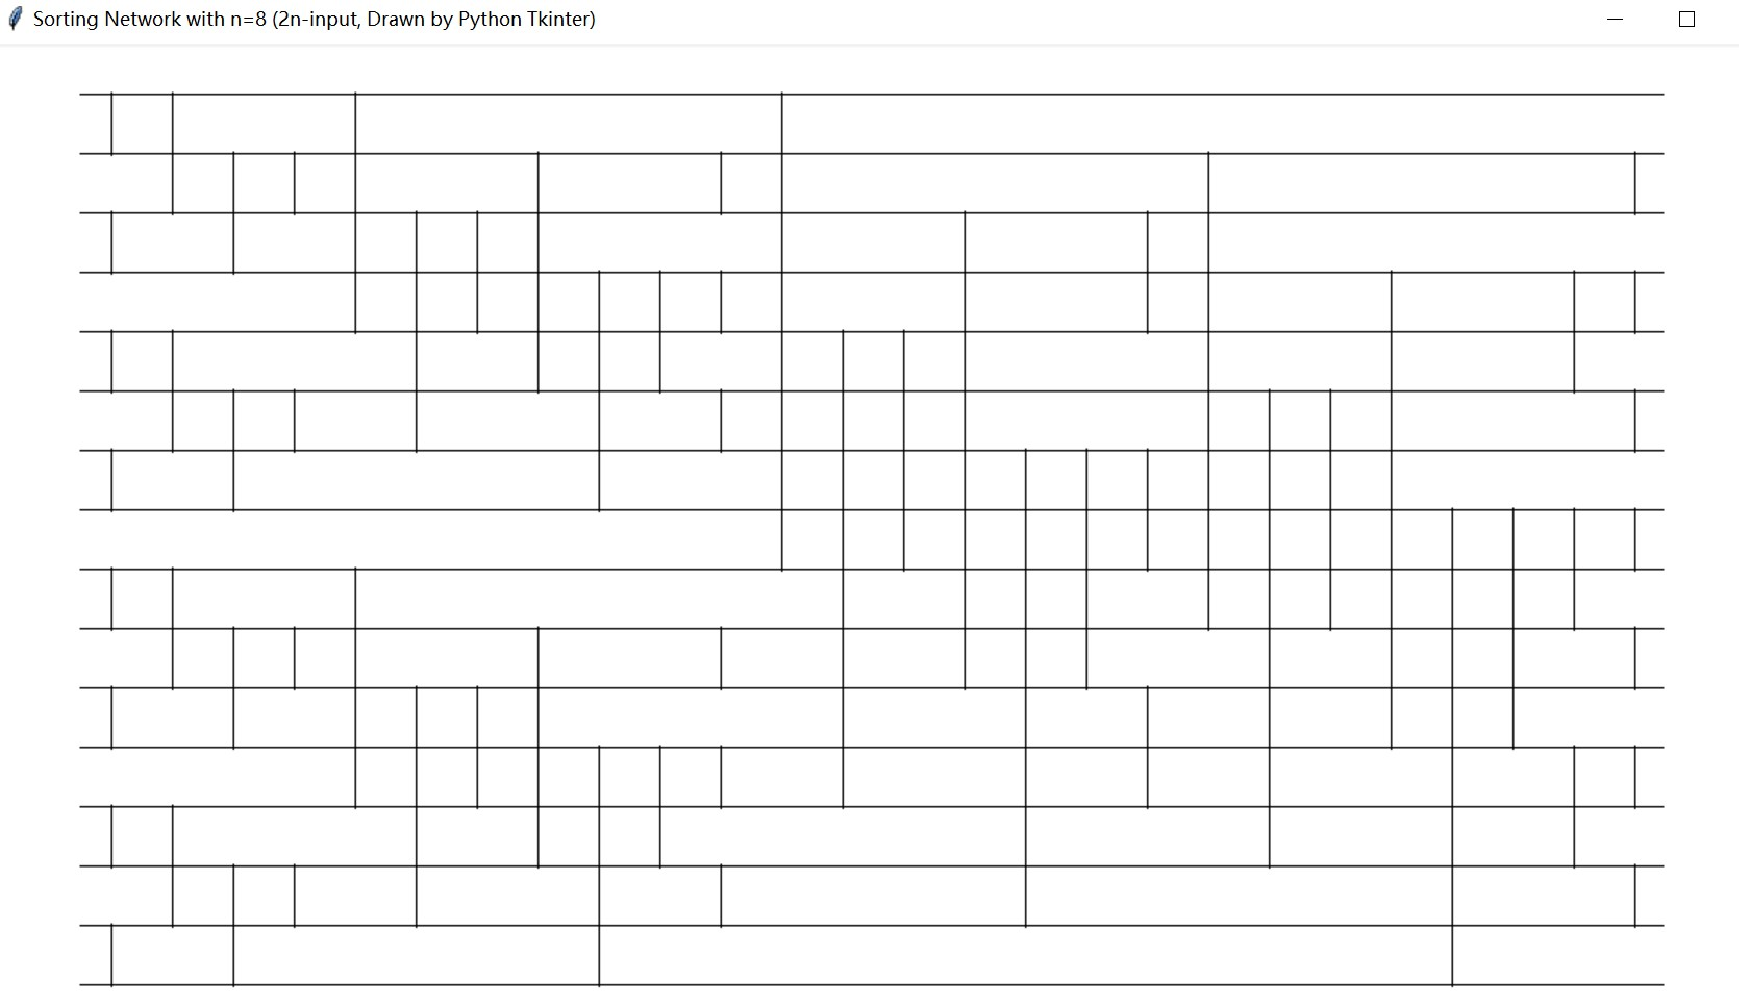
\includegraphics[width=0.99\textwidth]{8.pdf}
    			\caption*{\textbf{Fig.1} $n = 8$} \label{Fig-8}
    		\end{minipage}
    		\hspace{5mm}
    		\begin{minipage}[h]{0.52\textwidth}
    			\centering
    			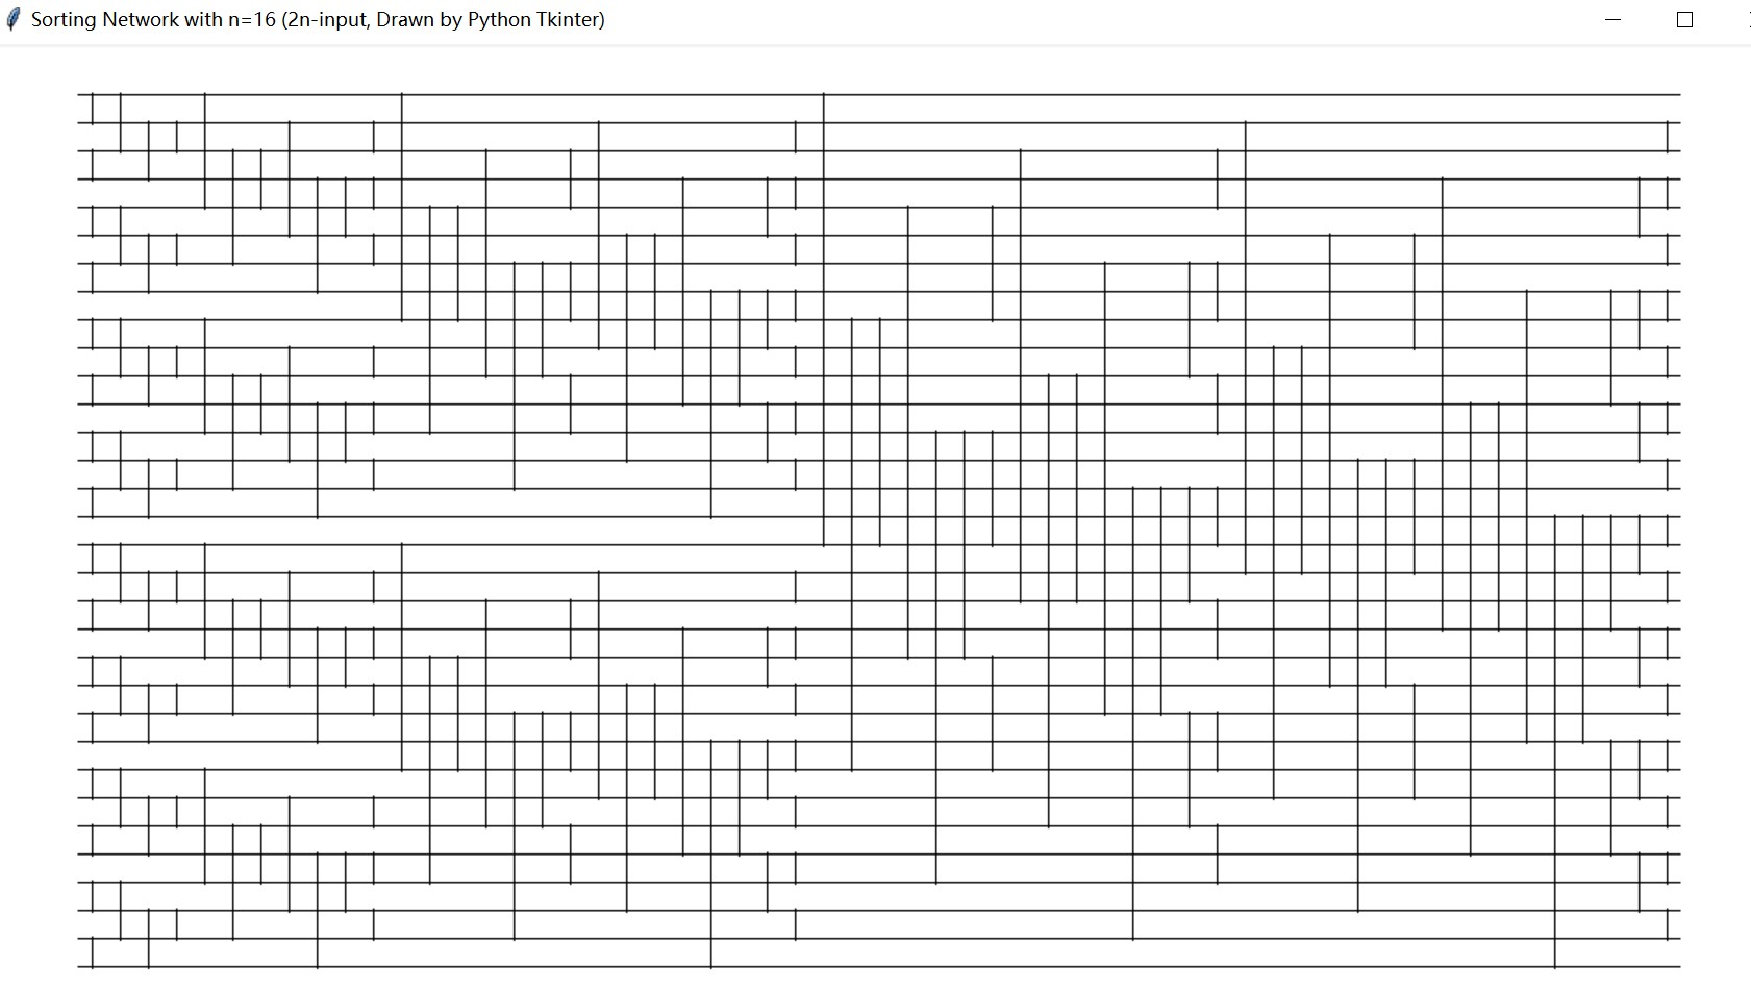
\includegraphics[width=0.99\textwidth]{16.pdf}
    			\caption*{\textbf{Fig.2} $n = 16$} \label{Fig-16}
    		\end{minipage}
    	\end{figure}
    
    	\begin{figure}[htbp]
    		\begin{minipage}[h]{0.48\textwidth}
    			\centering
    			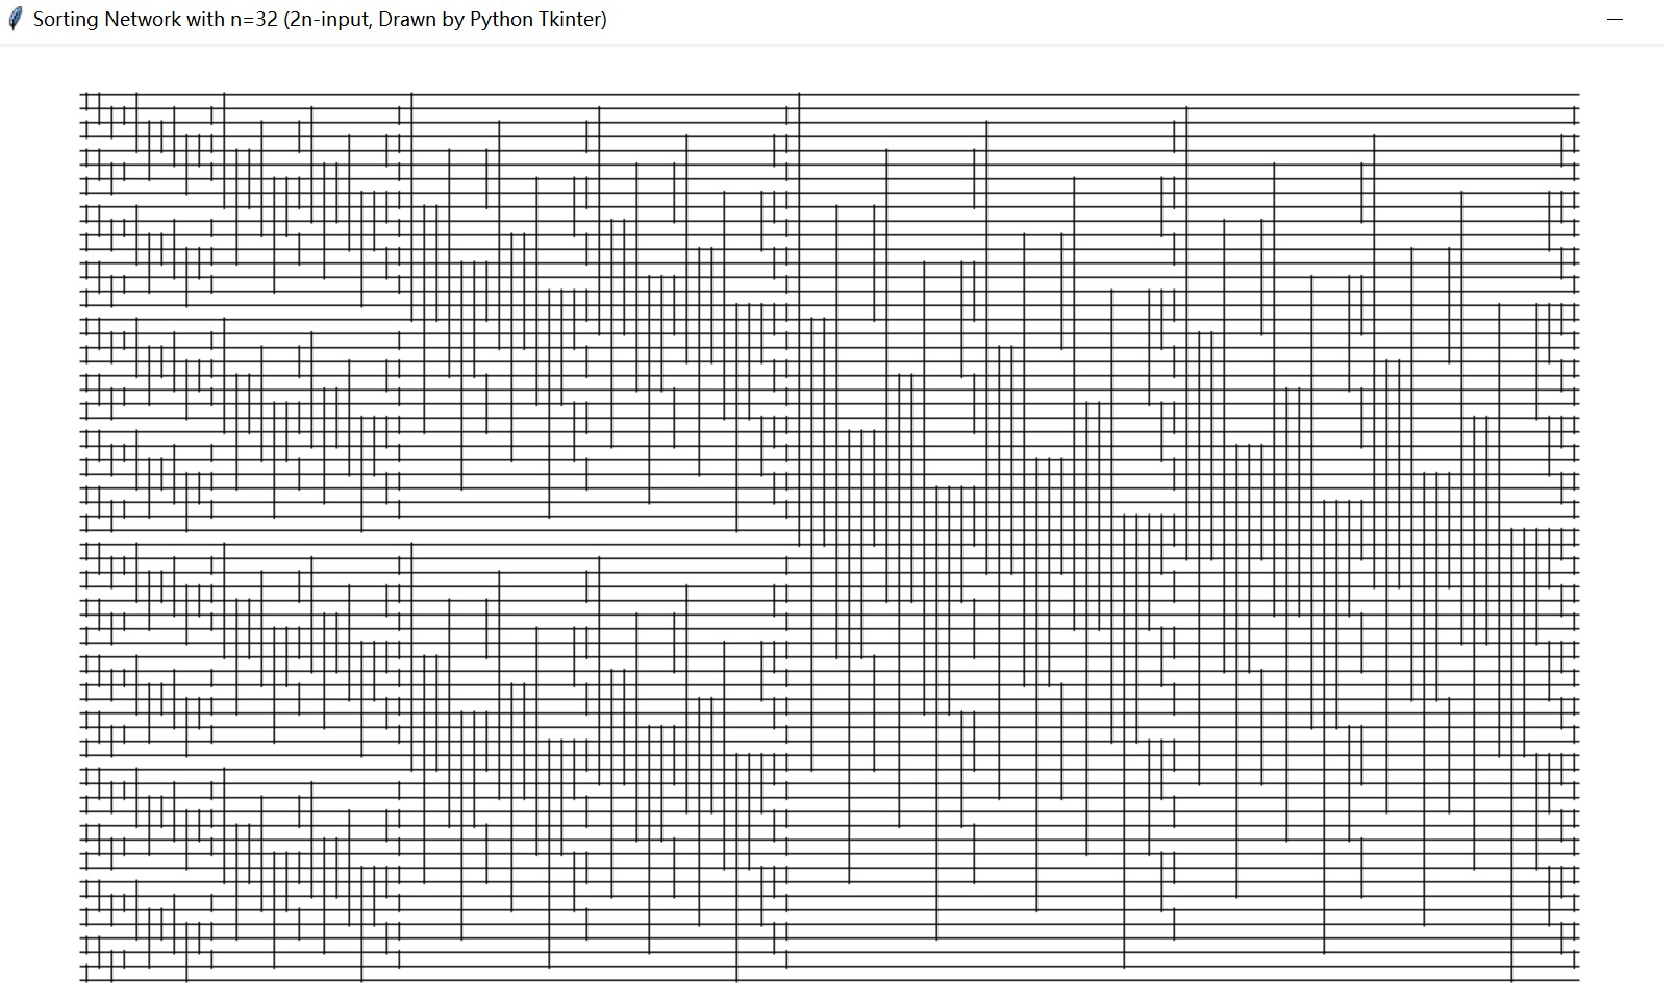
\includegraphics[width=0.99\textwidth]{32.pdf}
    			\caption*{\textbf{Fig.3} $n = 32$} \label{Fig-32}
    		\end{minipage}
    		\hspace{5mm}
    		\begin{minipage}[h]{0.54\textwidth}
    			\centering
    			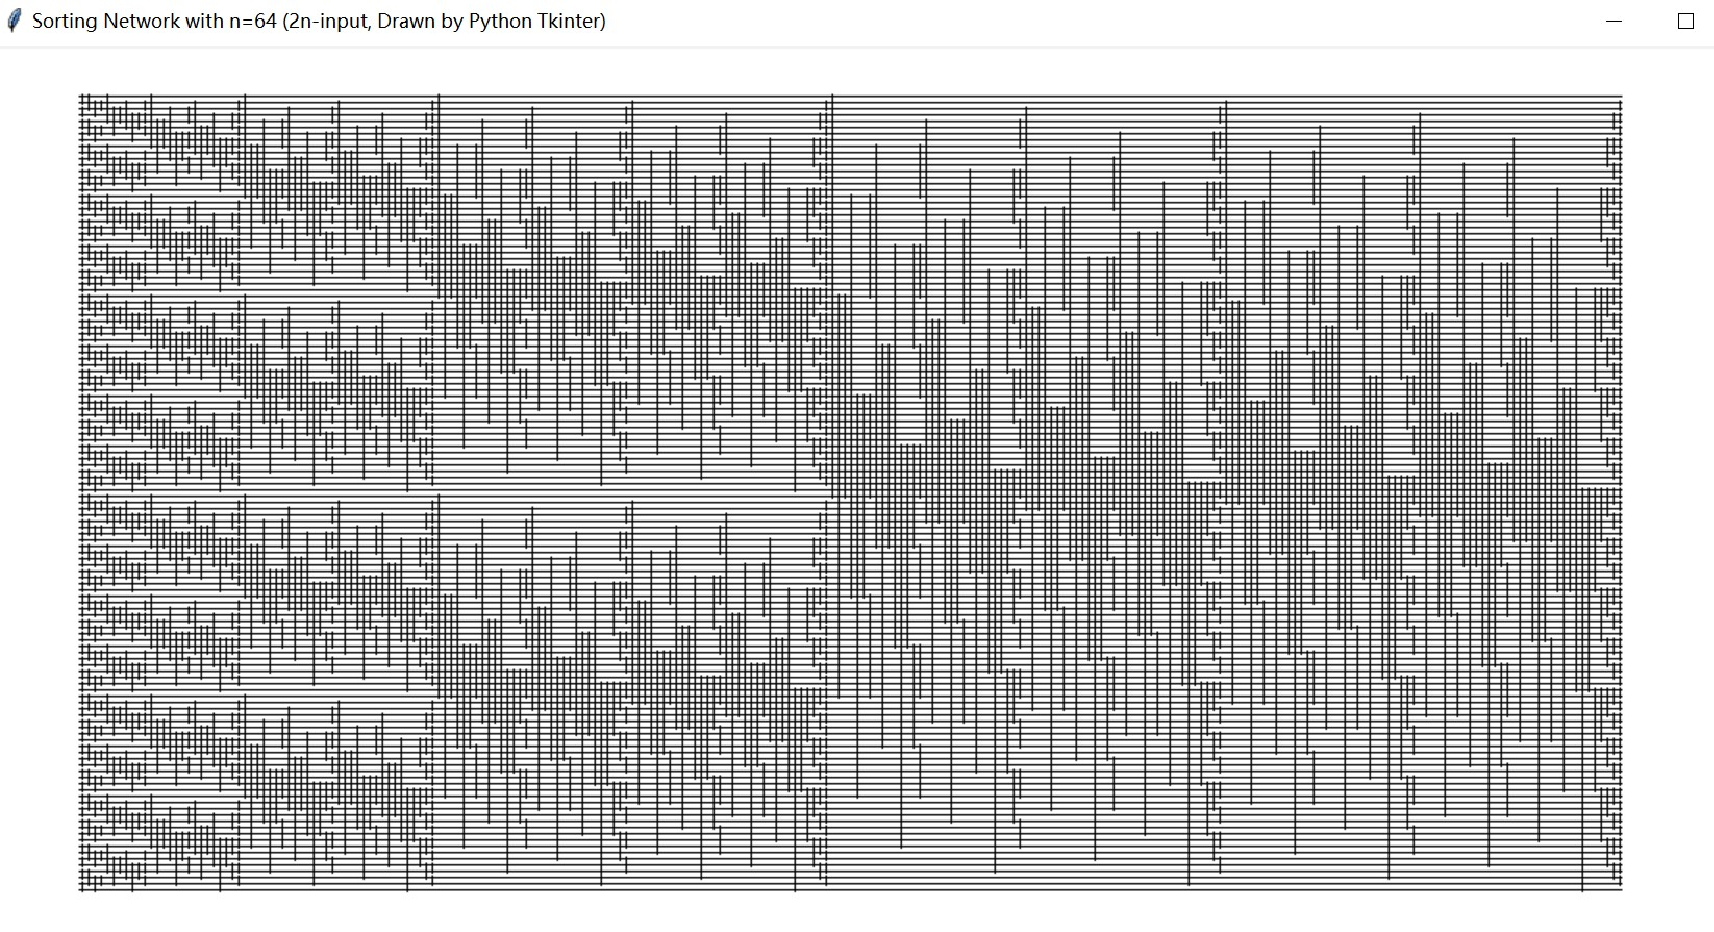
\includegraphics[width=0.99\textwidth]{64.pdf}
    			\caption*{\textbf{Fig.4} $n = 64$} \label{Fig-64}
    		\end{minipage}
    	\end{figure}	
    	\footnotesize{$*$ The \href{run:OddEvenSortingNetwork-YijiaDiao.py}{source code} lent part of the python code on the course website.}\\
    	
    	\item What is the depth of a $2n$-input odd-even sorting network?
    	\begin{solution}
    		Suppose the depth of odd-even merge operation is $ M(n) $, the depth of the network is $ D(n) $.Then we have:
    		\begin{align*}
    			M(n) = \begin{cases}
    			&1 ,\quad \text{if}\quad n = 1 \text{;}\\
    			&M(\frac{n}{2}) + 1 ,\quad \text{if}\quad n > 1 \text{;}\\
    			\end{cases}
    		\end{align*}
    		According to Master Theorem, $ M(n) = O(\log n) $.Since $ D(n) = D(\frac{n}{2}) + M(n) $, 
    		\begin{align*}
    			D(n) &= D(\frac{n}{4}) + O(\log \frac{n}{2}) + O(\log n)\\
    				 &= \cdots\\
    				 &= \sum_{i = 0}^{k} O(i), k = \log n\\
    				 &= O(k^2)\\
    				 &= O(\log^2 n)
    		\end{align*}
    		We can conclude that the depth of Batcher's odd-even merging network is $ O(\log^2 n) $.
    	\end{solution}
    	\item
    	{\color{red}{(Optional Sub-question with Bonus)}} Use the zero-one principle to prove that any $2n$-input odd-even merging network is indeed a merging network.
    	
    \end{enumerate}

\end{enumerate}

\vspace{20pt}

\textbf{Remark:} You need to include your .pdf, .tex and .py files (or other possible sources) in your uploaded .rar or .zip file.

%========================================================================
\end{document}
